% Chapter 1
\chapter{Eaglescience --Chapter01.tex} % Chapter title

\label{ch:Eaglescience} % For referencing the chapter elsewhere, use \autoref{ch:introduction} 

%----------------------------------------------------------------------------------------

Het hier beschreven onderzoek en daarbij behorende applicatie is geschreven in opdracht van Eaglescience wat gevestigd is in Amsterdam Sloterdijk. Eaglescience ontwikkeld complexe software op projectbasis voor diverse klanten vaak met een wetenschappelijke inslag. Het bedrijf telt +/- 20 medewerkers waarvan 75\% ontwikkelaar/designer zijn en de resterende 25\% een support rol bekleden (project managers finance manager, Quality manager)  Aan het hoofd van Eaglescience staat een CEO, Marc Grootjen, CTO Bas Breier, CFO Wender van Mansvelt. Naast het ontwikkelen van nieuwe software biedt Eaglescience ook de mogelijkheid om zorg te dragen voor de eventuele hosting van het opgeleverde product. Hiermee kan Eaglescience nog beter garanderen dat de geboden kwaliteit in de software gewaarborgd blijft tijdens de levensduur van de software.

\section{Organisatie}
Eaglescience bestaat uit drie divisies die elk onder Eaglescience B.V. vallen. Iedere divisie is verantwoordelijk voor een deel van die diensten die Eaglescience aanbied.
\begin{figure}[bth]
\myfloatalign
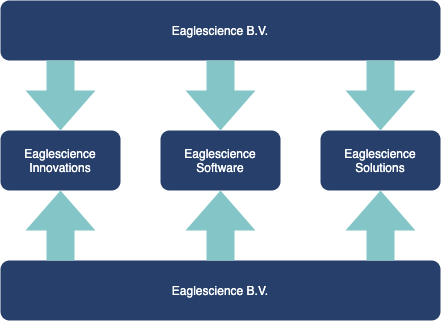
\includegraphics[width=10cm]{gfx/organogram}
\caption{Organogram Eaglescience}
\label{fig:Eaglescience organogram}
\end{figure}
\section{missie}
De missie van Eaglescience is het bedienen van onze partners door een ontwerp, ontwikkeling en service te bieden op het gebied van op maat gemaakte IT oplossingen . Om dit te kunnen bewerkstelligen heeft Eaglescience goed opgeleide IT professionals in dienst die zichzelf continue ontwikkelen op de “cutting edge” van IT technologie. De hoofd competenties van de medewerkers zijn: innovatief, intelligent, klant georientee\"erd, flexibel en ambitieus.
\section{visie}
Eaglescience streeft er als innovatief IT bedrijf naar om software te ontwikkelen als een Business-to-Business dienst. Met onze technische vaardigheden bouwen we veilige en hoogwaardige software die bijdraagt aan een betere wereld. Omdat we agile werken, leveren we precies wat nodig is, niets meer en niets minder. Wij helpen onze klanten zoeken naar een langdurige betrokkenheid en samenwerking op basis van zowel vertrouwen als wederzijds respect. Omdat elke vraag uniek is, ontwikkeld Eaglescience op maar gemaakte en innovatieve software. We zijn van plan deel uit te maken van het hele proces van het formuleren van een idee tot het lanceren van het product en het waarborgen van de productie levenscyclus. Onze belangrijkste succesfactor zijn de mensen, die zich continu ontwikkelen door met de nieuwste technieken te werken op diverse projecten. Wij streven naar een optimale balans tussen werk en priv\'e. Dit geeft onze medewerkers veel vrijheid, maar vereist zelfdiscipline en verantwoordelijkheid. 
\section{strategie}
\marginpar{strategische thema's}
Eaglescience levert de visie via vier strategische thema's:
\begin{itemize}
\item Maatschappelijke verantwoordelijkheid
\item Persoonlijke groei
\item Tevredenheid
\end{itemize}
We streven ernaar om veilige en hoogwaardige software diensten te leveren die waarde toevoegen aan onze samenleving. We streven naar een bedrijfscultuur waarin alle collega's hun talenten kunnen laten groeien. We hebben een ongecompliceerd werkethos: we richten ons op resultaten van hoge kwaliteit, maar met een gezonde balans tussen werk en priv\'e en voldoende tijd voor leuke en sociale evenementen. Eaglescience verwacht van alle medewerkers dat zij hun handelen baseren op vier kwaliteitsprincipes:
\begin{itemize}
\item Meld situaties die niet voldoen aan onze interne procedures
\item Evalueer risico's wanneer grote veranderingen worden verwacht
\item Help en daag elkaar uit
\item Kennis behouden over compliancy en kwaliteitsmanagement
\end{itemize} 
\section{Relevante en actuele ontwikkelingen binnen Eaglescience}
Eaglescience is aan het groeien, zowel in het aantal projecten waar aan gewerkt wordt als het aantal medewerkers. Daarnaast worden de diensten die Eaglescience aanbied ook uitgebreid. Waarbij het hosten van de ontwikkelde applicaties steeds meer wordt aangeboden. Door deze inzet ligt de verantwoordelijk niet alleen bij het leveren van een veilige en hoogwaardige software maar het leveren van service waarbij de applicaties in een veilige omgeving worden aangeboden. Mede door de groei van het bedrijf maar zeker ook de diensten die aangeboden wordt is het zeer relevant om taken die geautomatiseerd kunnen worden te automatiseren.
